%%%%%%%%%%%%%%%%%%%%%%%%%%%%%%%%%%%%%%%%%%%%%%%%%%%%%%%%%%%%%%%%%%%%%%%%%%%%%%%

\chapter{OS DADOS}

Como descrito na seção anterior, os dados aqui analisados dizem respeito ao fluxo solar no comprimento de onda de 10.7 cm que, junto com o número de manchas solares, é um dos dados de mais longo registro da atividade solar - o início sistemático de sua observação se deu em 1947 \cite{tapping201310}. Esta quantidade é expressa em unidades de fluxo solar (ou sfu, do inglês \textit{solar flux unit}), onde 1 sfu = 10$^{-22}$Wm$^{-2}$Hz$^{-1}$.

Os dados foram baixados de \url{https://omniweb.gsfc.nasa.gov/form/dx1.html}. Eles dizem respeito à série temporal de 28 de novembro de 1963 a 20 de julho de 2020. Para esta janela temporal, os seguintes dados foram baixados: média dos valores diários (Figura \ref{fig:dailyavg}), média de 27 dias (Figura \ref{fig:27dayavg}) e média anual (Figura \ref{fig:yearluavg}). As Figuras a seguir foram geradas automaticamente pelo portal de acesso aos dados.

%%%%%%%%%%%%%%%%%%%%%%%%%%%%%%%%%%%%%%%%%%%%%%%%%%%%%%%%%%
% DAILY AVERAGES
\begin{figure}[ht!]
	\caption{Médias diárias do índice F10.7.}
	\vspace{0mm}	% acrescentar o espaçamento vertical apropriado entre o título e a borda superior da figura
	\begin{center}
		\resizebox{13cm}{!}{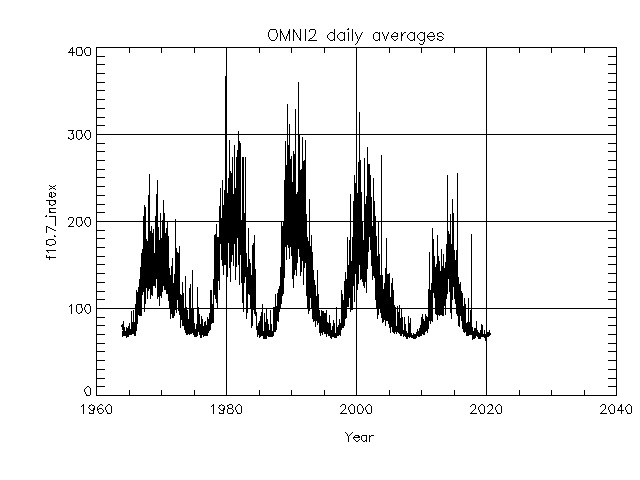
\includegraphics{Figuras/jpg_omni2_daily_wSxReptBqw.jpg}}		
	\end{center}
	\vspace{-2mm}	% acrescentar o espaçamento vertical apropriado entre a borda inferior da figura e a legenda ou a fonte quando não há legenda (o valor pode ser negativo para subir)
	\legenda{Médias das medições diárias do fluxo solar. Visualização fornecida pelo portal utilizado para download. Uma análise direta dos dados indicou presença de saltos com valores 999.9, denotando falhas na aquisição. Variações de grande amplitude ocorrem com maior frequência (diariamente), enquanto uma variação global de amplitude média ocorre na escala de alguns anos. O arquivo possui 20440 registros.}	% legenda - para deixar sem legenda usar comando \legenda{} (nunca deve-se comentar o comando \legenda)
	\label{fig:dailyavg}
	\FONTE{\url{https://omniweb.gsfc.nasa.gov/form/dx1.html}.}	% fonte consultada (elemento obrigatório, mesmo que seja produção do próprio autor)
\end{figure}

%%%%%%%%%%%%%%%%%%%%%%%%%%%%%%%%%%%%%%%%%%%%%%%%%%%%%%%%%%
% 27 DAY AVERAGES
\begin{figure}[ht!]
	\caption{Médias de 27 dias do índice F10.7.}
	\vspace{0mm}	% acrescentar o espaçamento vertical apropriado entre o título e a borda superior da figura
	\begin{center}
		\resizebox{13cm}{!}{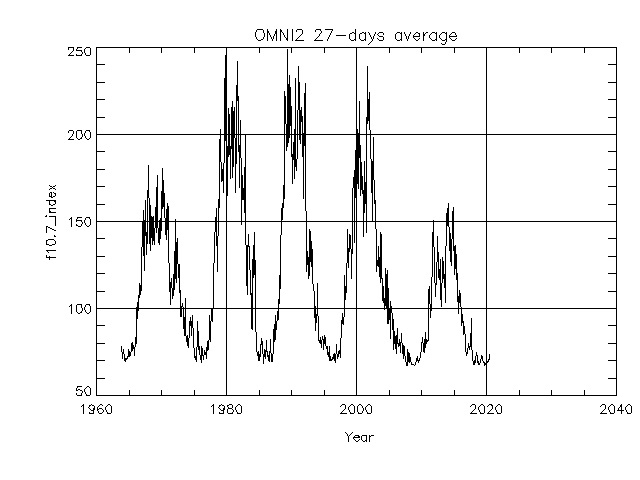
\includegraphics{Figuras/jpg_omni2_27day_bdhxX8pSxb.jpg}}		
	\end{center}
	\vspace{-2mm}	% acrescentar o espaçamento vertical apropriado entre a borda inferior da figura e a legenda ou a fonte quando não há legenda (o valor pode ser negativo para subir)
	\legenda{Médias de 27 dias. As médias tornam o sinal menos oscilatório em pequenas escalas. Ao todo são 672 medições.}	% legenda - para deixar sem legenda usar comando \legenda{} (nunca deve-se comentar o comando \legenda)
	\label{fig:27dayavg}
	\FONTE{\url{https://omniweb.gsfc.nasa.gov/form/dx1.html}.}	% fonte consultada (elemento obrigatório, mesmo que seja produção do próprio autor)
\end{figure}

%%%%%%%%%%%%%%%%%%%%%%%%%%%%%%%%%%%%%%%%%%%%%%%%%%%%%%%%%%
% YEARLY AVERAGES
\begin{figure}[ht!]
	\caption{Médias anuais do índice F10.7.}
	\vspace{0mm}	% acrescentar o espaçamento vertical apropriado entre o título e a borda superior da figura
	\begin{center}
		\resizebox{13cm}{!}{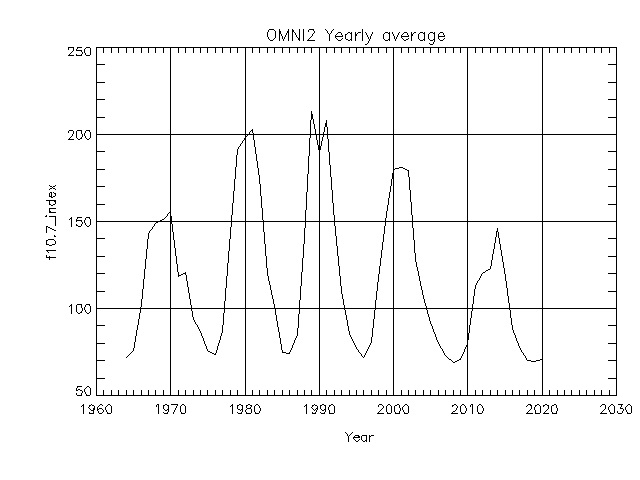
\includegraphics{Figuras/jpg_omni2_yearly_3G19RccK_m.jpg}}		
	\end{center}
	\vspace{-2mm}	% acrescentar o espaçamento vertical apropriado entre a borda inferior da figura e a legenda ou a fonte quando não há legenda (o valor pode ser negativo para subir)
	\legenda{Média anual. Novamente o sinal evidencia sua característica de longo prazo: uma variação sinusoidal com o período de alguns anos. O arquivo possui 56 registros.}	% legenda - para deixar sem legenda usar comando \legenda{} (nunca deve-se comentar o comando \legenda)
	\label{fig:yearluavg}
	\vspace{-3mm}
	\FONTE{\url{https://omniweb.gsfc.nasa.gov/form/dx1.html}.}	% fonte consultada (elemento obrigatório, mesmo que seja produção do próprio autor)
\end{figure}

\begin{figure}[ht!]
	\caption{Tratamento dos dados de média diária.}
	\vspace{0mm}	% acrescentar o espaçamento vertical apropriado entre o título e a borda superior da figura
	\begin{center}
		\resizebox{12cm}{!}{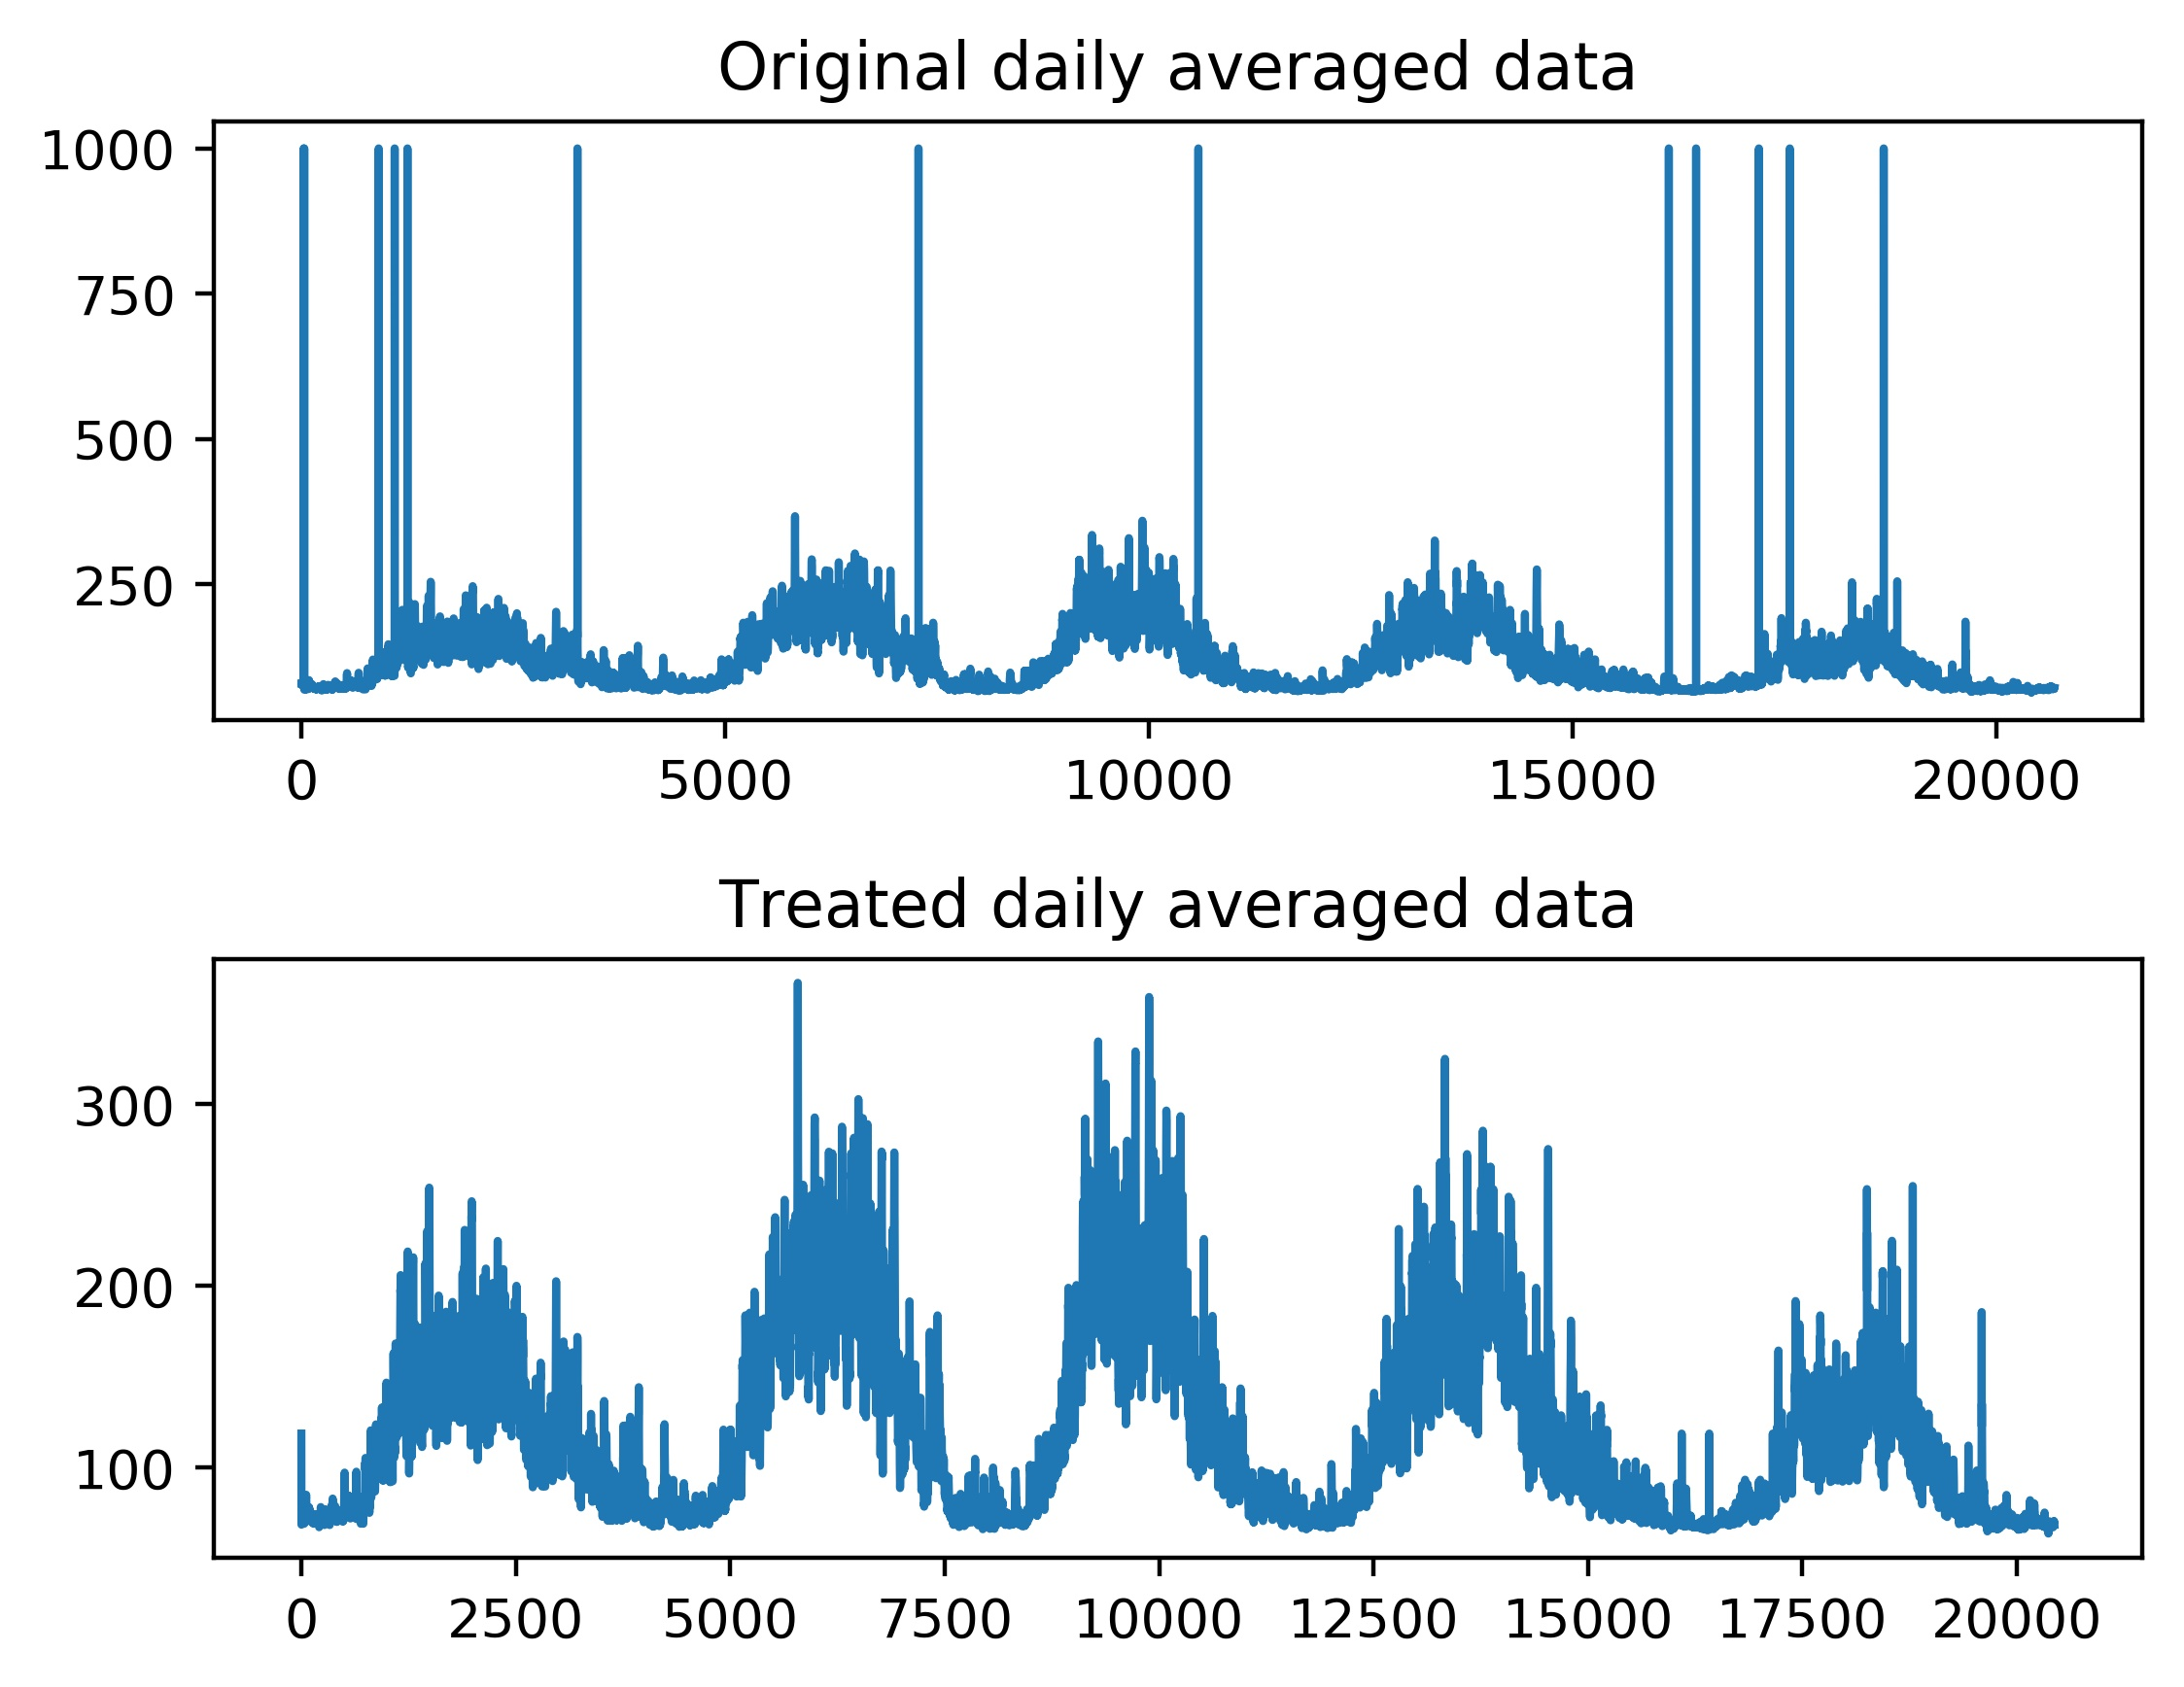
\includegraphics{Figuras/final_2.jpg}}		
	\end{center}
	\vspace{3mm}	% acrescentar o espaçamento vertical apropriado entre a borda inferior da figura e a legenda ou a fonte quando não há legenda (o valor pode ser negativo para subir)
	\legenda{Topo: dados de média diária do fluxo F10.7 conforme baixados, sem nenhum tipo de tratamento; abaixo: mesmos dados após os procedimentos (1), (2) e (3) descritos nesta seção. No plot de baixo, o limite do eixo vertical é reduzido para que um aspecto interessante do sinal possa ser observado: existe uma assimetria na série temporal, que aparenta crescer mais rapidamente e decrescer mais lentamente.}	% legenda - para deixar sem legenda usar comando \legenda{} (nunca deve-se comentar o comando \legenda)
	\label{fig:datavis}
	%\FONTE{\url{https://omniweb.gsfc.nasa.gov/form/dx1.html}.}	% fonte consultada (elemento obrigatório, mesmo que seja produção do próprio autor)
\end{figure}

Os dados diários (Figura \ref{fig:dailyavg}) apresentam valores iguais a 999.9, denotando um valor espúrio a ser lidado antes da análise. Outra característica deste dado é que, para cada ano, existem 365 ou 366 registros, a depender de ser ano bissexto ou não. Para os dados da média de 27 dias (Figura \ref{fig:27dayavg}), existem 13 ou 14 registros, a depender do ano (por motivos intrínsecos ao processo de aquisição dos dados e seus intervalos de medição). Os dados anuais (Figura \ref{fig:yearluavg}) possuem, como esperado, um registro para cada ano. Porém, os anos de 1963 e 2020 de todos os dados dizem respeito a registros incompletos destes anos (apenas de novembro a dezembro de 1963 e de janeiro a julho de 2020). 

Tendo em vista estas características, os dados foram tratados com a seguinte estratégia: (1) a série de 1964 a 2019 foi usada, ignorando-se os valores referentes a 1963 e 2020; (2) os valores 999.9 dos dados de média diária foram substituídos pela média da série; (3) 365 registros de cada ano foram usados nos dados de média diária, ignorando-se o registro extra dos anos bissextos; (4) 12 registros de cada ano foram usados nos dados de média de 27 dias, ignorando-se os demais; (5) o tamanho da série foi reduzida para a maior potência de dois entre zero e o tamanho da série. A Figura \ref{fig:datavis} exibe o dado de média diária antes e depois dos procedimentos (1), (2) e (3) descritos neste parágrafo. 